\documentclass[UTF8,fontset=fandol,11pt,a4paper]{ctexart}
\usepackage[margin=27mm]{geometry}
\usepackage{amsmath,amssymb,amsthm,mathtools,bm}
\usepackage{graphicx,booktabs,longtable,array,tabularx}
\usepackage[numbers,sort&compress]{natbib}
\usepackage{xcolor,hyperref}
\hypersetup{colorlinks=true,linkcolor=blue!45!black,citecolor=blue!45!black,urlcolor=blue!45!black}
\usepackage{microtype}
\xeCJKDeclareCharClass{CJK}{"2460 -> "2466}
\setlength{\emergencystretch}{2em}
\setlength{\parskip}{0.25em}
\newtheorem{theorem}{定理}[section]
\newtheorem{proposition}[theorem]{命题}
\newtheorem{lemma}[theorem]{引理}
\newtheorem{corollary}[theorem]{推论}
\theoremstyle{definition}
\newtheorem{definition}[theorem]{定义}
\newtheorem{condition}[theorem]{条件}
\theoremstyle{remark}
\newtheorem{remark}[theorem]{说明}
\newcommand{\e}{\mathrm e}
\newcommand{\ii}{\mathrm i}
\newcommand{\1}{\mathbf 1}
\newcommand{\CC}{\mathbb C}
\newcommand{\RR}{\mathbb R}
\newcommand{\ZZ}{\mathbb Z}
\newcommand{\QQ}{\mathcal Q}
\newcommand{\Cx}{\mathfrak C_x}
\newcommand{\ip}[2]{\langle #1,#2\rangle}
\newcommand{\norm}[1]{\left\|#1\right\|_2}
\DeclareMathOperator{\diag}{diag}
\DeclareMathOperator{\rank}{rank}
\DeclareMathOperator{\tr}{tr}
\DeclareMathOperator{\Ran}{Ran}

\title{孪生素数研究的七岛框架：\\精确结构、解析障碍与两类桥接问题\\[5pt]
\large A Seven-Island Framework for Twin-Prime Research:\\
Exact Structures, Analytic Obstructions, and Two Bridging Problems}
\author{}
\date{2026年9月12日\\统一研究母稿 v0.1}
\begin{document}
\pagestyle{plain}
\maketitle
\begin{abstract}
本文将固定移位素数对的研究材料，按算术基础、解析消去、固定原子、实际出现项结构、非自治动力学、孪生素数终点和几何辅助提升七个模块重新组织。目标是在同一对象、量词和归一化下，明确已成立的结构和仍需算术输入的转移。技术核心是一类保留单位掩码、平滑核和对角删除的实际算子：我们重述并证明其精确正形式分解、范数与行能量规模，以及实际系数范数对系数无关方法的限制。在区间尺度 $x$、素数模数尺度 $Q=x^{1/3}$ 下，低频压缩给出数量为 $(1/4+o(1))Q^2$ 的负方向；完整 Kloosterman 表达说明单侧短支撑不自动产生双侧临界区间节省。对于一个明确构造的平滑分割，边界贡献以 $xQ^2x^{-11/64+o(1)}$ 的代价整体移除。动力学部分通过中国剩余定理与 Abel 求和，重述实际移动筛事件的线性方差界及 Haar 几乎处处的无限命中结论，同时保留指定算术种子 $0$ 的未证回接条件。这些结果既不证明内部有符号算术消去，也不证明孪生素数猜想；它们构成可追溯的结构与障碍综整，将两类未完成的桥接问题从已有成果中分离出来。

\end{abstract}
\noindent\textbf{关键词：}孪生素数；Möbius相关；单位剩余类；Gram算子；Kloosterman和；指定初始点。
\clearpage
\setcounter{tocdepth}{1}
\tableofcontents
\clearpage
\section{引言：从分散局部结果到共同问题}
孪生素数问题要求在固定移位 $2$ 上证明无穷多个素数对。它并不只要求建立一个形式上类似相关和的表达式，也不只要求某个有限矩阵具有小范数。若一种方法把原始计数问题转移到新的载体，那么载体上的系数、支撑、量词与归一化必须一并转移；忽略其中任一项，可能得到一个正确但不能用于原问题的命题。

本研究档案包含编号 TPC1--TPC418 的多轮局部探索，以及若干原型、缺源标记和后续未编号研究。其形成过程是问题驱动的：一个表达式的障碍引出新的表达方式，一次源对应核查又要求重新辨认实际对象。把这些工作按编号顺次压缩，会保留探索顺序，却不一定保留数学逻辑。因此，本文以图~\ref{fig:map}为共同坐标，重建一条可独立阅读的论证，并把没有进入证明链的材料留在可追溯的补充索引中。

\begin{figure}[p]
\centering
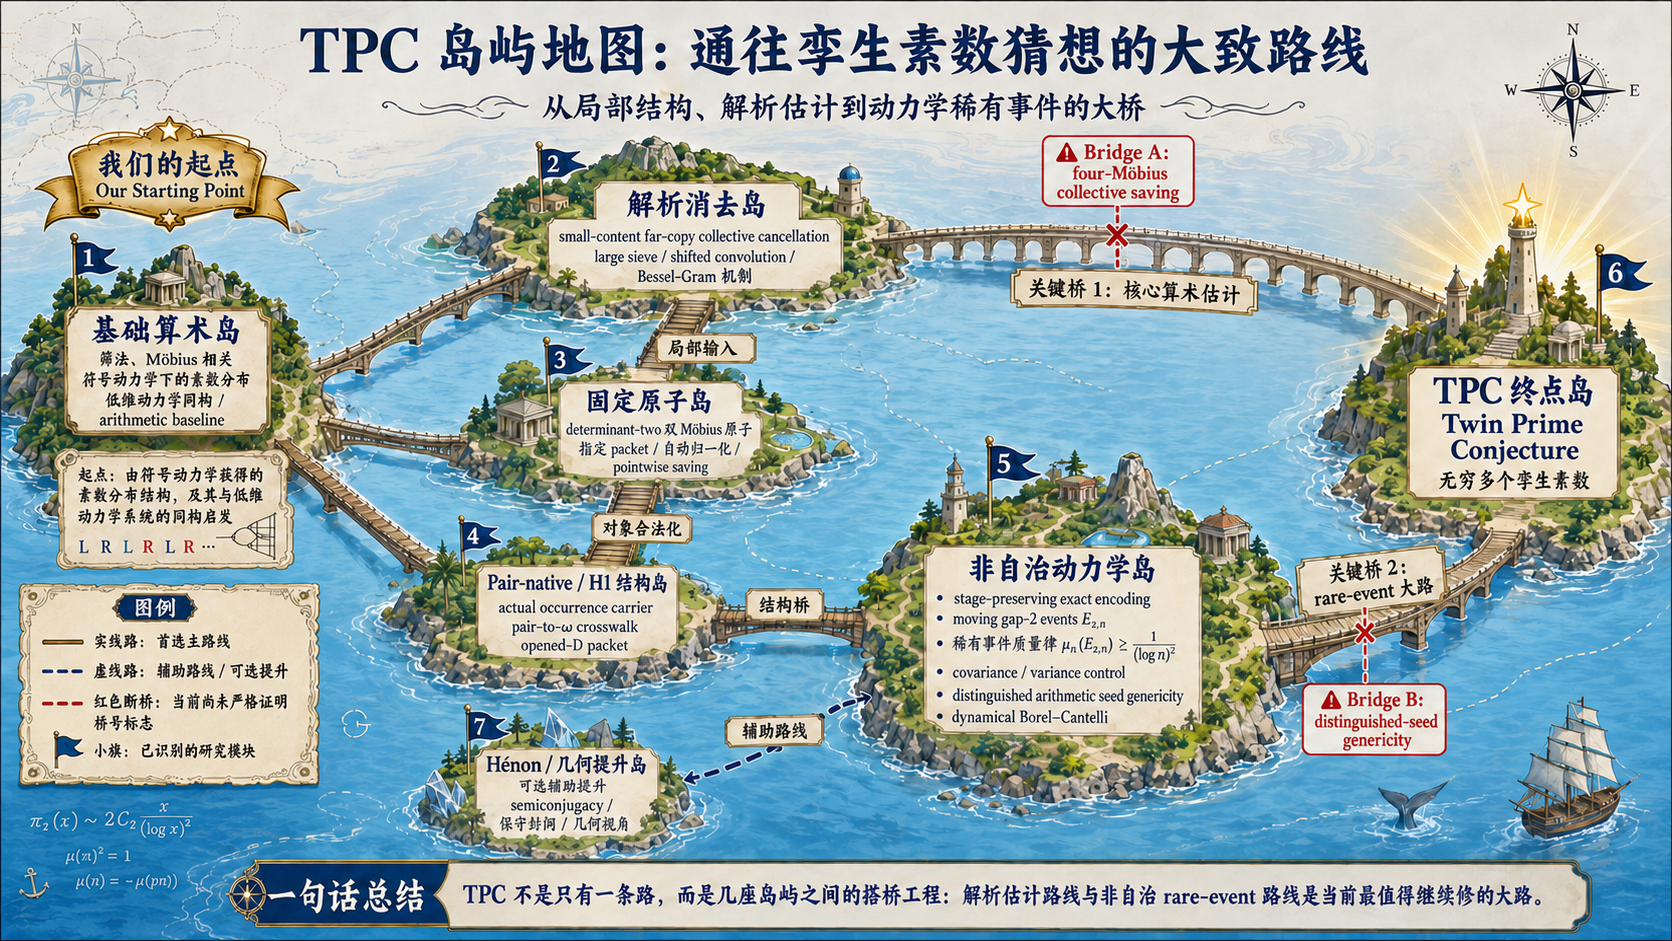
\includegraphics[width=\textwidth]{../../../research/tpc-big-road/figures/tpc_route_cn.png}
\caption{用户提供的七岛／两桥研究地图，原样复用。岛号表示研究对象与任务分工，不是已完成的步骤。实线为拟议主路线，虚线为辅助路线，红色断桥表示图示中的待证转移，不能解释为所有方法不可能。特别地，动力学岛所写的事件质量下界是该路线需要落实的条件，而非本文对指定算术轨道已经证明的事实。图像 Bridge A 内含档案中的 Gate A 与 Gate B；图像 Bridge B 是指定种子动力学桥，与文件名中的 Bridge-B 不同。小字宜放大查看；配套 README 提供全分辨率原图入口。}
\label{fig:map}
\end{figure}

\subsection{一个框架，两种实质缺口}
解析路线从局部相关结构走向完整的有符号集体消去。本文固定讨论的一个目标量具有自然尺度 $xQ^2$；要成为既定端点契约的有效输入，需要严格超过 $1/400$ 的幂次节省。完整恒等式可以保证对象不被改变，但不会凭空提供这种节省。第三、四岛分别处理指定局部原子和实际出现项的合法对应，第二岛才承担相应估计。

动力学路线的困难不同。即使一个编码系统具有足够的事件质量和协方差控制，也仍须证明被原始算术问题指定的那条轨道位于良好点集。关于几乎所有初始点的结论，不包含任意预先指定点。这一量词缺口不能通过改称“典型轨道”消除。几何提升若只改变表示方式，也不能替代该输入。

\subsection{本文保留的核心结果}
本文围绕四组可以逐项检查的内容展开：
\begin{enumerate}
\item 在明确的固定移位系数、单位剩余类和核约定下，证明实际算子的精确分解与行能量规模，而不把模型矩阵当作原始算子。
\item 证明常向量范数下界、实际系数的范数下界与增长维数的低秩修补障碍，明确它们限制的是哪些上界方法，而不是原混合标量的大小。
\item 用完整 Kloosterman 恒等式及一短一完整数组的精确范数，分离代数表达、支撑压缩和有符号重组三项义务。
\item 构造一个具有统一导数控制的分割，并在原混合标量层面支付边界代价；把剩余内部估计和动力学种子回接列为未完成条件。
\end{enumerate}
动力学部分另给出实际移动筛事件的 $O(N)$ 方差界与 Haar 几乎处处无限命中证明；它与指定种子 $0$ 的未证结论分开陈述。这些是已有档案结果的统一陈述与证明重组，不在本文中宣称首次发现或最优性。早期有限证书与后续模型增长结果在附录中按证据类型区分，不被误计为实际算术收益。

\subsection{与既有数学输入的关系}
本文的素数计数输入是经典素数定理及其分部求和推论\cite{selberg1949}。混合系数的二阶矩估计使用 Mertens 乘积定理的无条件基线；文献\cite{lamzouri2015}的开头提供该基线的陈述，本文不使用其中关于偏差分布的条件性结论。频率分离、正半定压缩、有限 Fourier 正交和谱极小极大原理是结构证明中的标准工具，其使用不构成新的素数对定理。

Blomer--Pascadi 的临界区间双线性估计\cite{blomer2026}提供一种有用的外部基准：在正确长度与互素条件下，Kloosterman 双线性型具有局部幂次节省。本文只使用其定理~1.1在平方根长度处的专门化，并检查本研究的表达是否真的满足这类输入条件；不把外部定理的存在等同于完整物理表达的估计已经完成。

本文不是该领域文献的穷尽综述，也不以内部资料数量代替与外部文献的创新性比较。它是一份限定研究计划的数学综整母稿。正式投稿之前，仍须进行贡献定位、补充相关文献、核验选用的全部历史依赖，以及独立的全文数学审查。

\subsection{阅读路径}
第~\ref{sec:arithmetic}节给出共同目标和证据层次；第~\ref{sec:structure}节解释局部原子与实际载体；第~\ref{sec:operator}--\ref{sec:boundary}节是自足的解析核心。动力学与几何路线在第~\ref{sec:dynamics}节单独处理，两桥的条件账本在第~\ref{sec:bridges}节汇总。读者不需要依次阅读所有历史小稿才能理解正文；但精确出处、未选用材料及审核范围可在配套来源矩阵和全目录索引中查找。

\section{共同算术目标、量词与路线分工}\label{sec:arithmetic}
\subsection{终点与辅助量}
记 $\pi_2(y)=\#\{p\le y:p,p+2\text{ 均为素数}\}$。终点是 $\pi_2(y)\to\infty$，不是有限区间内找到更多素数对。一个常用加权辅助量是
\[
S_2(y)=\sum_{n\le y}\Lambda(n)\Lambda(n+2),
\]
其中 $\Lambda$ 是 von Mangoldt 函数。若证明某个正主项规模的渐近式，例如 $S_2(y)\sim c y$ 且 $c>0$，则可推出孪生素数无穷；这里的渐近式只是充分条件，本文没有证明它。

这一蕴含需要排除真素数幂的贡献。至少一个坐标为 $p^k$、$k\ge2$ 的整数对有 $O(\sqrt y\log y)$ 个，每项权重至多 $O(\log^2 y)$，总贡献为 $o(y)$。若真素数对只有有限多个，剩余加权贡献也不可能形成正的线性主项。这个初等核查提醒我们：即使辅助量是标准形式，其与终点的连接也应写出来，而不能只借助命名。

\subsection{岛①：局部筛因子为何还不是素数对计数}
令 $y\ge2$，$P_y=\prod_{p\le y}p$、$s_y(n)=\1_{(n,P_y)=1}$、$\rho_y=\prod_{p\le y}(1-1/p)$。
对固定有限非空的互异整数移位集 $\mathcal H=\{h_1,\ldots,h_r\}\subset\ZZ$，记 $\nu_p(\mathcal H)$ 为其模 $p$ 的不同剩余类数。
CRT 给出完整周期的精确恒等式
\[
C_y(\mathcal H):=\frac1{P_y}\sum_{n\bmod P_y}\prod_{h\in\mathcal H}s_y(n+h)
=\prod_{p\le y}\left(1-\frac{\nu_p(\mathcal H)}p\right).
\]
证明只需逐素数数出 $p-\nu_p(\mathcal H)$ 个允许类，再由 CRT 相乘。
若 $\mathcal H$ 可容许，即每个 $\nu_p<p$，则对足够大的 $p$ 有 $\nu_p=r$，
归一化局部因子 $(1-r/p)(1-1/p)^{-r}=1+O_r(p^{-2})$，因此乘积收敛。
特别对 $\{0,2\}$，
\[
\frac{C_y(\{0,2\})}{\rho_y^2}\longrightarrow 2C_2,\qquad
C_2=\prod_{p>2}\frac{p(p-2)}{(p-1)^2}>0.
\]
这是经典局部计算，不是本研究新得到的素数对渐近式\cite{archive1}。

将 $\min\mathcal H$ 平移为零并记 $h_{\max}=\max\mathcal H$，令 $X\to\infty$。
若 $Y_X=\sqrt{X+h_{\max}}$ 且 $Y_X<n\le X$，则所有 $n+h$ 均大于 $Y_X$、不超过 $Y_X^2$。
它们通过 $Y_X$ 以下素数筛，当且仅当它们都是素数。这是\emph{逐点识别}，没有估计通过筛的数量。
另一方面，对完整的 $1\le n\le X$ 窗口，周期分割只给出
\[
\left|\sum_{1\le n\le X}\prod_{h\in\mathcal H}s_y(n+h)-XC_y(\mathcal H)\right|
\le P_y+1.
\]
因为完整周期的贡献精确，余下不足一个周期的部分误差至多 $P_y$，非整数端点再付 $1$。
当 $P_y=o(X\rho_y^r)$ 时，上述周期截断界保证归一化误差趋于零；
而在精确识别尺度 $y=Y_X$ 上，素数定理给出 $\log P_{Y_X}\sim\sqrt X$，
故这一误差上界不能提供所需的相对误差控制。
这只是两种初等论证适用尺度不相接，不是所有筛方法的不可能定理。

\subsection{七岛不是单一串行证明}
\begin{table}[ht]
\centering\small
\caption{七岛的数学分工。表中“尚需”不是对全部可能路线的必要性断言。}
\begin{tabularx}{\textwidth}{c l X}
\toprule
岛 & 对象或任务 & 在本框架中尚需辨认的转移\\
\midrule
1 & 算术基础 & 从筛法、相关量或编码出发，保留原始计数解释\\
2 & 解析消去 & 从局部结构到完整实际系数的有符号节省\\
3 & 固定原子 & 指定移位、指定相位与固定 packet 的逐点控制\\
4 & 实际出现项／H1 & 完整载体、来源对应、重数与逐系数守恒\\
5 & 非自治动力学 & 从测度命题到指定算术初始点的命中结论\\
6 & 孪生素数终点 & 无穷多个真实素数对，而非模型或有限证书\\
7 & 几何辅助提升 & 保时对应与事件读出，不额外获得算术典型性\\
\bottomrule
\end{tabularx}
\end{table}

\subsection{每次转移携带的契约}
为比较来自不同阶段的公式，本文把一个来源契约记为
\[
\mathcal O=(\text{系数},h_0,\text{支撑与顺序},\text{参数范围},
\text{量词},\text{归一化},\text{损失预算}).
\]
这不是一个新增数学对象，而是防止误用定理的记录方式。两个公式符号相似，并不表示它们的 $\mathcal O$ 相同。例如，任意大的 CRT 起点不等于给定物理区间内的起点；在一组完整壳层上的前缀不等于任意素数删选；重新计算局部行能量也不等于压缩原有归一化矩阵。

本文使用四种证据表述。第一种是可以直接展开验证的有限恒等式；第二种是带有完整假设与证明的统一命题；第三种是明确保留未证前提的条件推论；第四种是有限数值诊断。数值诊断不承担无限量词，条件推论不会因它的程序检查通过而变成无条件定理。本文后续的每个命题都应按这一层次阅读，而非按它在研究档案中出现的先后阅读。

\section{固定原子与实际出现项：岛③和岛④}\label{sec:structure}
这一层的任务不是先估计一个方便的代用品，而是确定下游估计必须作用于哪个对象。固定移位、固定相位、固定模数和固定支持是四种不同的要求。

\subsection{行列式二的保序拉回}
取整数区间 $I$，正整数 $a,s$，整数 $d,u$，满足
\[
\begin{gathered}
D(z)=d+sz>0,\quad V(z)=u+az>0\quad(z\in I),\quad su-ad=2,\\
(a,s)=1,\quad(as,2)=1,\quad(d,s)=(u,a)=1.
\end{gathered}
\]
以 $\lambda$ 表示 Liouville 函数，区别于后面的截断投影权。设 $B,\tau$ 为已指定整数，$\chi,W_X$ 为原块指定的函数。字面系数为
\[
a_{\xi,X}(z)=\mu(D(z))\mu(V(z))\1_{(B,V(z))=1}
\chi(\tau+Bz)W_X(\tau+Bz).
\]
\begin{proposition}[保留掩码的精确变换]\label{prop:pullback}
令 $q_{\rm prog}=as$，$n(z)=su+as z=sV(z)=aD(z)+2$。
它是 $I$ 到其像 $\mathcal N_I$ 的保序双射，而且
\begin{align*}
\mu(D(z))\mu(V(z))
&=\lambda(q_{\rm prog})\lambda(n-2)\lambda(n)\mathcal Q_{a,s}(n),\\
\mathcal Q_{a,s}(n)&=\mu^2((n-2)/a)\mu^2(n/s).
\end{align*}
因此任意相位 $\alpha\in\RR$ 下，原和精确等于
\[
\sum_{z\in I}a_{\xi,X}(z)\e(-\alpha z)
=\lambda(q_{\rm prog})\sum_{n\in\mathcal N_I}
\lambda(n-2)\lambda(n)\mathcal Q_{a,s}(n)
\mathcal W_{\xi,X}(n)\e(-\alpha z(n)),
\]
其中 $\mathcal W_{\xi,X}(n)=\1_{(B,n/s)=1}\chi(\tau+Bz(n))W_X(\tau+Bz(n))$。
每一个初始前缀也满足同样的等式。
\end{proposition}
\begin{proof}
$as>0$ 给出保序性；$su-ad=2$ 给出两个整数商。由
$\mu(m)=\mu^2(m)\lambda(m)$ 及 $\lambda$ 的完全乘法性，
$\lambda(n-2)\lambda(n)=\lambda(a)\lambda(s)\lambda(D(z))\lambda(V(z))$。
再乘 $\lambda(as)$，其平方等于 $1$，即得系数恒等式。其余因子原样代入，
不取绝对值也不删除平方自由掩码。保序双射将每个前缀映为对应前缀。
\end{proof}
这是 TPC127 的核心接口\cite{archive127}。它也保留沿相邻像点计算的变差和绝对比较质量，但并未估计这些量。固定 $h_0=2$ 不保证跨尺度固定一个相位，亦不允许删去商的平方自由条件。

\subsection{有序对、子项重组与出现项守恒}
平方展开所产生的是有序行对。它与上面一对仿射形式不是同一个载体。
例如 opened-$D$ 构造中 $N_\alpha(j)=\ell_\alpha d_\alpha j+h_0$，非对角对的系数含
\[
\mu(d_\alpha)\mu(d_\gamma)(\log\ell_\alpha)(\log\ell_\gamma)
r_R(N_\alpha(j))r_R(N_\gamma(j))B_\alpha(j)B_\gamma(j).
\]
这里 $r_R$ 与 $B_\alpha$ 是源展开的截断因子和行权别名；本稿不把它们另定义为可自由选择的函数，也不据此声称生产对已映入某个仿射原子。完整源公式见来源矩阵中的 TPC18；对到保留原子的附接仍需原有联合掩码、调度和归一化。

对于已经合法保留的源项，约数分解有一个简洁的守恒恒等式。令 $G>0$，
\[
\lambda_G(v)=\sum_{g\mid v,\ g\le G}\mu(v/g).
\]
则对正整数 $d,e$，
\[
\sum_{v\mid(d,e)}\lambda_G(v)=\1_{(d,e)\le G}.
\]
证明是交换 $g,v$ 后使用 $\sum_{h\mid m}\mu(h)=\1_{m=1}$。
这说明需要\emph{全部子项的带权和}来重组源项；一个子项不等于源系数。
TPC93 的逆变换和符号重组是在其平方自由、primitive 支持上成立的；TPC205 的生产对复合仍以合法附接为条件\cite{archivestructure}。

线性的出现项提升又是另一个问题。源标签 $\mathsf{EPS}$ 表示 eligible-prefix-soft（可用前缀的软分支），
$\mathsf{ETO}$ 表示 eligible-tail-open（可用尾部的开放分支），
$\mathsf{FUM}$ 表示 frontier-unmapped（前沿未映射分支）。
非软域为 $\mathcal C=\mathcal C^{\mathsf{ETO}}\sqcup\mathcal C^{\mathsf{FUM}}$，不能只保留前沿而删掉尾部。
若上游分割满足
\[
\1_{\mathsf{EPS}}^TM^{\mathsf{EPS}}+\1_{\mathcal C}^TM^{\rm ns}
=\1_{\mathcal N}^T,
\]
且一个已提供的提升 $L:\CC^{\mathcal C}\to\CC^{\mathcal O}$ 满足
$\1_{\mathcal O}^TL=\1_{\mathcal C}^T$，则相乘便得
\[
\1_{\mathsf{EPS}}^TM^{\mathsf{EPS}}+\1_{\mathcal O}^TLM^{\rm ns}
=\1_{\mathcal N}^T.
\]
其中 $\mathcal N,\mathcal C,\mathcal O$ 分别是原生项、非软分支、带来源路径的保留出现项载体。
保留载体不是已认证非零的 active support：后者还需对逆聚合后的字面系数作非零认证，不能将未求值的系数直接判零。
这个条件命题不构造 $L$；还需逐行分离、元数据保真与非零实际系数支持。形式支持包络不能代替实际出现项集。

\subsection{带权覆盖的可检验判据}
设已给定实际系数向量 $c_{\rm phys}$ 和合法块合成矩阵 $B$，两侧均使用指定的正定内积。令 $B^\dagger$ 为相应 Moore--Penrose 逆，$P=BB^\dagger$。
\begin{proposition}[覆盖与正交障碍]
在有限维空间中，以下条件等价：
\[
c_{\rm phys}\in\operatorname{Ran}B,\qquad Pc_{\rm phys}=c_{\rm phys},\qquad
\langle y,c_{\rm phys}\rangle=0\quad(y\in\ker B^*).
\]
且到可合成空间的距离等于
\[
\|(I-P)c_{\rm phys}\|=
\max_{y\in\ker B^*,\ \|y\|\le1}|\langle y,c_{\rm phys}\rangle|.
\]
\end{proposition}
\begin{proof}
奇异值分解说明 $P$ 是到 $\operatorname{Ran}B$ 的正交投影，而其正交补为 $\ker B^*$。
正交分解给出三个等价条件。Cauchy--Schwarz 给出距离公式的上界；残差非零时取其单位化向量得到等号，残差为零时两侧均零。
\end{proof}
这是 TPC117 判据的线性代数内容\cite{archivestructure}。即使 $B^\dagger c_{\rm phys}$ 是精确覆盖系数，若各块上界为 $U_b$，传输仍要支付
$\sum_b|(B^\dagger c_{\rm phys})_b|U_b$。
覆盖存在与覆盖廉价不是一回事；更不是实际增长族的算术节省。

\section{解析核心：实际算子的定义与精确结构}\label{sec:operator}
本节至第~\ref{sec:boundary}节采用同一对象，来自已恢复完整来源的标量契约\cite{archivev59,archivephysical}。这里“物理”仅指原研究问题实际指定的算术数据，用来与可自由选择符号、起点和核的模型区分。

\subsection{参数、系数和核}
令 $x\to\infty$，并置
\[
I_x=(x/2,x]\cap\ZZ,\quad N=\lfloor x\rfloor-\lfloor x/2\rfloor,\quad
Q=x^{1/3},\quad H=x^{21/32},\quad U=x^{133/400}.
\]
旧来源的尺度是 $x=2X$，故 $N=X+O(1)$。令 $\QQ=\{q\text{ 为素数}:Q<q\le2Q\}$。固定 $K>0$，取 $z=(\log x)^K$，定义
\begin{align}
P(z)&=\prod_{p\le z}p,&
W_z&=\prod_{p\le z}\frac p{p-1},&
C_z&=\prod_{p>z}\left(1-\frac1{(p-1)^2}\right),\nonumber\\
b_x^{(z)}(u)&=\1_{I_x}(u)C_zW_z\1_{(u+2,P(z))=1}
 \prod_{\substack{p\mid u\\p>z}}\frac{p-1}{p-2},\label{eq:hybrid}\\
\beta(t)&=\frac{\Lambda(t)}{\log t}-\sum_{\substack{d\mid t\\d\le U}}\mu(d),\nonumber\\
w(u)&=\Lambda(u+2)-b_x^{(z)}(u).\label{eq:lanes}
\end{align}
所有 $x$ 充分大，使 $z\ge2$。$K$ 先固定再取阈值，不作 $K$ 随 $x$ 增长的断言。低素数乘积含素数 $2$，禁余类是 $-2$；$\beta$ 中的 $\mu$ 是 Möbius 函数。两个实际系数向量都为实数，但可具有变化的符号。

固定一个非负、实值、光滑函数 $\psi_+$，支撑于 $[-1,1]$ 且积分为 $1$。记 $\e(t)=\exp(2\pi\ii t)$，
\[
\kappa(y)=\int_{\RR}\psi_+(v)\e(-vy)\,dv,\qquad K_H(h)=\kappa(h/H).
\]
不要求 $\psi_+$ 偶对称，因此 $\kappa$ 未必实值；但 $\kappa(-y)=\overline{\kappa(y)}$、$\kappa(0)=1$。它是 Schwartz 函数，而非在 $|h|>H$ 时严格为零的核。旧正号 Fourier 约定通过反射 $\psi_+(v)=\psi(-v)$ 与此一致。

\subsection{完整标量与行能量}
令 $a_q=q/(q-1)$，在 $\ell^2(I_x;\CC)$ 上定义
\[
A_q(u,t)=a_q\kappa((u-t)/H)
 \big((q-1)\1_{q\mid u-t}-1\big)
 \1_{q\nmid u}\1_{q\nmid t}\1_{u\ne t},\qquad A=\sum_{q\in\QQ}A_q.
\]
采用 $\ip fg=\sum\overline f g$ 的内积约定。目标标量为
\begin{equation}
\Cx=\ip w{A\beta}
=\sum_{q\in\QQ}q
 \sum_{\substack{u,t\in I_x\\u\ne t,\ q\nmid ut}}
 w(u)\beta(t)K_H(u-t)
 \left(\1_{u\equiv t\ (q)}-\frac1{q-1}\right).
\label{eq:scalar}
\end{equation}
外面的 $q$ 已含在矩阵定义中，不能再乘一次。$A$ 是 Hermitian 矩阵，但两个实向量的混合标量仍可能为复数。

所研究的行能量是
\[
G(u)=\sum_{q\in\QQ}\sum_{t\in I_x}|A_q(u,t)|^2,\quad
D_G=\diag(G(u)),\quad Z=D_G^{-1/2}AD_G^{-1/2}.
\]
它先对每个素数取平方，不含跨素数交叉项。只要全部 $G(u)>0$，
\begin{equation}
\Cx=\ip{D_G^{1/2}w}{Z D_G^{1/2}\beta}.
\label{eq:readout}
\end{equation}
因此，归一化算子范数变小不等于原标量变小；两个加权向量的代价必须同时计入。

\subsection{单位剩余类修正}
\begin{proposition}[精确正形式分解]\label{prop:decomp}
令 $r_q(n)=q\1_{q\mid n}-1$，并定义
\begin{align*}
T(u,t)&=\kappa((u-t)/H)\sum_{q\in\QQ}\sum_{a=1}^{q-1}\e(a(u-t)/q),\\
R(u,t)&=\kappa((u-t)/H)\sum_{q\in\QQ}\frac{r_q(u)r_q(t)}{q-1},\\
\Delta(u)&=\sum_{q\in\QQ}a_q(q-2)\1_{q\nmid u}.
\end{align*}
则 $A=T-R-\diag\Delta$，且
\[
R\ge0,\qquad 0\le A+\diag\Delta\le T
\]
为正半定序关系。
\end{proposition}
\begin{proof}
先在模 $q$ 的剩余类上令
\[
F_q(r,s)=q\1_{r=s}-1,\qquad
S_q(r,s)=a_q\big((q-1)\1_{r=s}-1\big)\1_{r\ne0}\1_{s\ne0}.
\]
当两个剩余类都非零、恰一个为零、或两个都为零时，$F_q-S_q$ 分别等于
$1/(q-1)$、$-1$、$q-1$，故
\[
F_q-S_q=\frac{r_qr_q^*}{q-1}.
\]
此外，$F_q/q$ 是全剩余类均值零子空间的正交投影，$S_q/q$ 是在零剩余类消失且在单位剩余类上和为零的子空间投影，故 $0\le S_q\le F_q$。

沿 $I_x\to\ZZ/q\ZZ$ 拉回保持正半定序，不要求各剩余类出现次数相同。对对角矩阵 $D_v(n,n)=\e(-vn/H)$，
\[
[\kappa((u-t)/H)S_q(u,t)]_{u,t\in I_x}
=\int\psi_+(v)D_vS_qD_v^*\,dv .
\]
非负权积分仍保持正半定序。对素数求和，并删除逐行精确对角
$S_q(n,n)=a_q(q-2)\1_{q\nmid n}$，得到结论。
\end{proof}
删除对角后的 $A$ 不必正半定。后面的负方向正是对角删除后的现象；若在重组中丢掉 $\Delta$，便改变了问题。

\section{范数规模、实际系数代价与低秩障碍}\label{sec:barriers}
\subsection{频率分离给出的上界}
固定常数 $B_\psi,B_\kappa<\infty$ 使
\[
0\le\psi_+(v)\le B_\psi(1+|v|)^{-2},\qquad
|\kappa(y)|\le B_\kappa(1+|y|)^{-2}.
\]
\begin{lemma}\label{lem:upper}
对 $Q\ge2$，
\[
\norm A\le4B_\psi(H+4Q^2)+3Q^2.
\]
\end{lemma}
\begin{proof}
不同约分分数 $a/q$ 在单位圆上至少相隔 $(4Q^2)^{-1}$，跨越零点的间隔亦然。定义在全部整数上的卷积核
$\kappa(h/H)\sum_{q,a}\e(ah/q)$ 的 Fourier 乘子为
\[
m(\theta)=H\sum_{q,a}\sum_{k\in\ZZ}
 \psi_+\big(H(a/q-\theta-k)\big)\ge0 .
\]
这由固定 Schwartz 核的 Poisson 求和得到。右边各点的实轴间距至少为
$s=H/(4Q^2)$；每个半开单位区间含点不超过 $1+1/s$。分割正负半轴并求和
$(1+j)^{-2}$，得到 $m(\theta)\le4B_\psi H(1+1/s)$。
压缩到 $I_x$ 后范数不增加。命题~\ref{prop:decomp}给出
$\norm{A+\diag\Delta}\le\norm T$，而
$\max\Delta<\sum_{Q<q\le2Q}q\le3Q^2$，故结论成立。
\end{proof}
由于 $H<Q^2$，实际尺度上 $\norm A\ll_\psi Q^2$。这一上界不使用 $\beta,w$ 的消去。

\subsection{所有实际行的能量}
\begin{proposition}\label{prop:energy}
对固定核和所有充分大的 $x$，一致于每个 $u\in I_x$，
\[
G(u)\asymp_\psi \frac{HQ^2}{\log Q}.
\]
\end{proposition}
\begin{proof}
连续性与 $\kappa(0)=1$ 给出固定 $0<\rho,b\le1$，使 $|\kappa(y)|\ge b$ 于 $|y|\le\rho$。在 $q\nmid u$ 时令
\[
S_q(u)=\sum_{\substack{t\in I_x\\t\ne u,\ q\nmid t}}|\kappa((u-t)/H)|^2,\quad
C_q(u)=\sum_{\substack{t\in I_x\\t\ne u,\ q\mid u-t}}|\kappa((u-t)/H)|^2.
\]
平方展开得到精确式
\[
G(u)=\sum_{\substack{q\in\QQ\\q\nmid u}}
 a_q^2\big(S_q(u)+(q-1)(q-3)C_q(u)\big).
\]
积分比较给出 $S_q(u)\le2B_\kappa^2H/3$、
$C_q(u)\le2B_\kappa^2H/(3q)$。因为 $1+(q-1)(q-3)/q\le q$，
每个素数的上界为 $(2B_\kappa^2/3)a_q^2qH$。

当 $N-1\ge2\rho H$ 且 $H\ge2Q/\rho$ 时，每行至少一侧含
$\lfloor\rho H/q\rfloor\ge\rho H/(2q)$ 个非零的同余差。这些点仍为单位剩余类，
且 $(q-2)^2\ge q^2/9$，所以该素数的贡献至少为
$(\rho b^2/18)a_q^2qH$。

任何 $u\le x=Q^3$ 至多有两个大于 $Q$ 的不同素因子。因此从
$S_Q=\sum_{q\in\QQ}a_q^2q$ 中因 $q\mid u$ 删除的质量至多 $9Q$。
素数定理和分部求和给出
$S_Q\sim(3/2)Q^2/\log Q$。在一个共同阈值后 $S_Q\ge18Q$，从而
\[
\frac{\rho b^2}{36}HS_Q\le G(u)\le\frac{2B_\kappa^2}{3}HS_Q
\]
对全部实际行成立。
\end{proof}
区间上界 $u\le Q^3$ 在这个论证中不可删除；这不是任意巨大起点上的同长度区间定理，也不是任意坐标前缀的行能量定理。

\subsection{常向量见证与实际系数}
\begin{theorem}[系数无关范数方法的障碍]\label{thm:normbarrier}
对第~\ref{sec:operator}节的固定数据，
\[
\norm A\ge(3/2+o(1))\frac{Q^2}{\log Q},\qquad
\norm w^2\sim\frac x2\log x,\qquad
\norm\beta^2\ge\left(\frac12\log\frac{27}{22}+o(1)\right)\frac x{\log x}.
\]
因此
\[
\liminf_{x\to\infty}\frac{\log Q}{xQ^2}
 \norm A\,\norm\beta\,\norm w
\ge\frac34\sqrt{\log(27/22)}>0.
\]
任何仅用 $B_x\norm\beta\norm w$ 且 $B_x\ge\norm A$ 的上界证明，都不能单独支付固定正幂次节省。
\end{theorem}
\begin{proof}
令 $f=N^{-1/2}\1_{I_x}$。未删对角的正形式为
\[
\ip f{(A+\diag\Delta)f}
=\frac1N\sum_q q\int\psi_+(v)V_q(v/H)\,dv ,
\]
其中 $V_q(\alpha)$ 是各单位剩余类上
$\sum_{n\equiv r(q),\,n\in I_x}\e(\alpha n)$ 减去其单位剩余类均值后的平方和，
不再除以 $q-1$。写 $I_x=\{a+1,\ldots,a+N\}$、$N=mq+s$，$0\le s<q$，并定义
\[
G_m(y)=\sum_{k=0}^{m-1}\e(ky),\qquad
S_j(\alpha)=\e(\alpha(a+j))
\bigl(G_m(\alpha q)+\1_{j\le s}\e(\alpha mq)\bigr),\quad 1\le j\le q.
\]
$S_j$ 就是剩余类 $a+j$ 上的和，包含 $m$ 个完整周期加至多一个末项。当
$0<|\alpha|q\le1/2$ 时，
\[
|G_m(\alpha q)|\le(2|\alpha|q)^{-1},\qquad
|\e(\alpha j)-1|\le2\pi|\alpha|q,\quad 1\le j\le q.
\]
故各和距一个共同中心不超过 $\pi+1$，在 $\alpha=0$ 时不超过 $1$。
减去均值最小化平方距离，得到 $V_q(\alpha)\le q(\pi+1)^2$。
由于核的频率支撑固定且 $2Q/H<1/2$ 最终成立，整个积分都在这个范围内。
正形式于是为 $O(Q^3/(N\log Q))=O(1/\log Q)$。
另一方面，单位整数数目 $N_q=N(1-1/q)+O(1)$ 给出
\[
\ip f{Af}=-\sum_{q\in\QQ}(q-2)+O(1/\log Q).
\]
素数定理与分部求和推出所述算子下界。

为控制 $w$，令
$c(p)=((p-1)/(p-2))^2-1=O(1/p)$，并在无平方因子整数上乘法延拓。
展开非负 Euler 乘积，去掉至多为 $1$ 的掩码，并扩大区间，得到
\[
\norm{b_x^{(z)}}^2
\le xW_z^2\prod_{p>z}(1+c(p)/p)\ll xW_z^2.
\]
乘积收敛，因为 $c(p)/p=O(p^{-2})$。Mertens 乘积定理给出
$W_z\ll\log z\ll_K\log\log x$。素数定理又给出
$\sum_{u\in I_x}\Lambda(u+2)^2\sim(x/2)\log x$；
真素数幂贡献为低阶项。三角不等式的双向范数比较即证明 $w$ 的渐近式，
不需假定 $b_x^{(z)}$ 与 $\Lambda$ 正交。

为控制 $\beta$，取素数
$x^{2/5}<p\le x^{9/20}$ 和 $x/(2p)<r\le x/p$。
最终 $p<r$ 且二者均大于 $U$，故 $n=pr\in I_x$、$\Lambda(n)=0$，
且 $n$ 在 $U$ 以下唯一的约数是 $1$，所以 $\beta(n)=-1$。
较小素因子唯一，计数不重复。普通二倍区间的素数定理在此范围内一致，故这些乘积数目为
\[
(1+o(1))\frac x2\sum_{x^{2/5}<p\le x^{9/20}}\frac1{p\log(x/p)}
=\left(\frac12\log\frac{27}{22}+o(1)\right)\frac x{\log x}.
\]
最后一步由分部求和和
$\int_{2/5}^{9/20}[a(1-a)]^{-1}\,da=\log(27/22)$ 得到。
将三个下界相乘即得结论。
\end{proof}

\begin{corollary}\label{cor:normalized}
对所定义的行能量归一化，
\[
H^{-1}\ll_\psi\norm Z\ll_\psi(\log Q)/H.
\]
而 $\norm Z\,\norm{D_G^{1/2}\beta}\,\norm{D_G^{1/2}w}$
仍至少为 $c_\psi xQ^2/\log Q$，其中 $c_\psi>0$。
\end{corollary}
\begin{proof}
由 $A=D_G^{1/2}ZD_G^{1/2}$，
$\norm A/G_{\max}\le\norm Z\le\norm A/G_{\min}$。
两个加权向量各自至少引入 $\sqrt{G_{\min}}$，
故其范数乘积上界表达至少为
$(G_{\min}/G_{\max})\norm A\norm\beta\norm w$。
应用命题~\ref{prop:energy}和定理~\ref{thm:normbarrier}即可。
\end{proof}
这里得到的是\emph{一个上界表达式的下界}，不是 $|\Cx|$ 的下界。
它不排除实际两系数之间的消去，也不排除其他预条件化或系数敏感方法。

\subsection{增长维数的负方向}
\begin{theorem}[低秩修补的限定障碍]\label{thm:rank}
置 $\tau_x=Q^2/\log Q$，
\[
J_x=\left\lfloor N\left(\frac1{4Q}-\frac1H\right)\right\rfloor,\quad
d_x=2J_x+1,\quad k_x=d_x-35.
\]
对全部充分大的 $x$，存在复子空间 $W_x$，使
\[
\dim_\CC W_x\ge k_x,\qquad
\ip f{Af}\le-\frac{\tau_x}{2}\norm f^2\quad(f\in W_x).
\]
特别地，任何复秩小于 $k_x$ 的矩阵 $E$，即使非 Hermitian，也满足
$\norm{A-E}\ge\tau_x/2$，且
$k_x=Q^2/4-x^{11/32}+O(1)$。
\end{theorem}
\begin{proof}
令 $U_0=A+\diag\Delta\ge0$，并取
$f_j(n)=N^{-1/2}\e(jn/N)$，$|j|\le J_x$。
这些向量在 $N$ 个连续整数上正交；最终 $d_x<N$。
对全部 $q\le2Q$ 与 $|v|\le1$，
$q|j/N+v/H|\le1/2$。前证的剩余类方差界于是给出
\[
\ip{f_j}{U_0f_j}\le\frac{C_0}{N}\sum_q q^2,\qquad C_0=(\pi+1)^2.
\]
令 $F$ 以这些向量为列，$B=F^*U_0F\ge0$，$M_1=\sum_q q$，则
\[
\tr B\le C_0(1+2Q/N)M_1.
\]
另一方面，任一实际整数至多被两个壳层素数整除，所以
\[
\Delta(n)\ge D_*:=\sum_q\frac{q(q-2)}{q-1}-4Q
\sim\frac32\tau_x .
\]
$B$ 中大于 $D_*/2$ 的特征值数目至多 $2\tr B/D_*<35$，最终同时有
$D_*\ge\tau_x$。取 $B$ 的 $[0,D_*/2]$ 谱子空间经 $F$ 映射后的空间为 $W_x$。
它丢失至多 $35$ 个维度，并且其 $U_0$ 二次型不超过 $D_*/2$，
而被删除对角至少为 $D_*$。这证明负性断言。
若 $\rank E<k_x$，则 $W_x\cap\ker E$ 非零；在其中取单位向量即得
$\norm{A-E}\ge|\ip f{(A-E)f}|\ge\tau_x/2$。
用 $N=x/2+O(1)$ 展开 $d_x$ 得到维数渐近式。
\end{proof}
这一谱截断不意味着整个低频带都为负，也不声称某个更高秩阈值以上就能成功。

若要求实见证，不能直接把复谱子空间改称实空间。
在同一对称频带改用 $f_0$、$(f_j+f_{-j})/\sqrt2$、
$(f_j-f_{-j})/(\ii\sqrt2)$ 组成实正交矩阵 $V$。
实对称矩阵 $\operatorname{Re}(V^*U_0V)$ 正半定，且迹等于 $\tr B$。
对它重复谱截断，得到不同的实子空间，维数仍至少 $k_x$。
具体地，对于实线性映射
\[
E:\RR^{I_x}\longrightarrow\CC^{I_x},\qquad \rank_{\RR}E<k_x,
\]
在该实负空间与 $\ker E$ 的交中取单位向量，便得到
$\|A-E\|_{\RR^{I_x}\to\CC^{I_x}}\ge\tau_x/2$。
这里范数使用实定义域的 Euclidean 单位球，秩指实像空间的维数，不能与复秩混用。
等式 $f^TAf=f^T\operatorname{Re}(A)f$ 只适用于同一个实向量的二次型，
不能用来把两个不同实际系数的 $w^TA\beta$ 替换成 $w^T\operatorname{Re}(A)\beta$。

\section{从精确发射到双侧短数组：不能省略的代价}\label{sec:emitter}
\subsection{完整 Kloosterman 表示}
设 $\eta_b$ 为第~\ref{sec:boundary}节构造的实分割函数，定义有限的物理标签集
\[
\mathcal J_x=\{j\in\ZZ:\operatorname{supp}\eta_{j,H}\cap[x/2,x]\ne\varnothing\},
\qquad |\mathcal J_x|=O(x/H+1).
\]
本节所有有序块对及其求和均限定于 $(b,c)\in\mathcal J_x^2$，并令
$a^{(j)}(t)=\eta_b(t)\beta(t)+\ii^j\eta_c(t)w(t)$，$j=0,1,2,3$。
固定 $q\in\QQ,v\in\RR$，定义单位剩余类上的和及其中心化
\[
F_r^{(j)}=\sum_{t\in I_x,\ t\equiv r(q)}a^{(j)}(t)\e(vt/H),\qquad
F_r^{(j),0}=F_r^{(j)}-\frac1{q-1}\sum_{s\ne0}F_s^{(j)}.
\]
在零剩余类令中心化向量为零。省略上标 $j$ 时，令
\[
\alpha_m=\frac1q\sum_{r\ne0}F_r^0\e(-mr/q),\quad
\gamma_n=\frac1q\sum_{r\ne0}\overline{F_r^0}\e(-n\bar r/q),\quad 1\le m,n<q,
\]
其中 $\bar r$ 是模 $q$ 的乘法逆元。
\begin{proposition}[发射恒等式与饱和]\label{prop:emitter}
对非归一化 Kloosterman 和 $S(m,n;q)=\sum_{r\ne0}\e((mr+n\bar r)/q)$，
\[
\mathcal B=\sum_{m,n=1}^{q-1}\alpha_m\gamma_nS(m,n;q)
=\sum_{r\ne0}|F_r^0|^2
=q\norm\alpha\norm\gamma.
\]
\end{proposition}
\begin{proof}
中心化使两个 Fourier 变换的零频率都为零。打开 $S$ 并分别作有限 Fourier 反演，两个内和恢复 $F_r^0$ 与 $\overline{F_r^0}$。Parseval 给出
$\norm\alpha^2=\norm\gamma^2=q^{-1}\norm{F^0}^2$，因为取逆是单位剩余类上的置换。
\end{proof}
这是精确表示，不是消去估计。数组范围为 $q-1$；即使已中心化，也没有得到 $\sqrt q$ 长度。例如 $F^0=e_1-e_2$ 的第一数组每个非零频率都非零。这个例子只检验接口，不认定实际算术向量就是它。

\subsection{先带符号重组，再处理残差}
记
\[
d_j(q)=\frac{q-2}{q-1}\sum_{t\in I_x,\ q\nmid t}|a^{(j)}(t)|^2,\qquad
E_{bcq}=\int\psi_+(v)\frac14\sum_{j=0}^3\ii^j[\mathcal B_j-d_j(q)]\,dv.
\]
直接展开四个平方，使用 $\sum_j\ii^j=\sum_j\ii^{2j}=0$，得
\begin{equation}
\Cx=\sum_{b,c}\sum_{q\in\QQ}qE_{bcq}.\label{eq:polarreturn}
\end{equation}
积分中的相位是 $\e(v(t-u)/H)$，与第~\ref{sec:operator}节核的方向一致。
减去 $d_j$ 精确删掉对角；外面的 $q$ 不可重复计入。四个正包各自可能饱和，而带符号组合仍可能消去。把它们先分别绝对化会丢失这一区别。

对支撑在整数区间且在 $q$ 的倍数处取零的数组，记
\[
\mathcal B_q(A_1,A_2)=\sum_{m,n}A_1(m)A_2(n)S(m,n;q).
\]
此处始终使用单位乘子 $1$，不随分解指标改变。
Blomer--Pascadi 的定理在两个整数区间长度均不超过常数倍 $\sqrt q$、单位乘子且满足其互素条件时，给出临界尺度界
\begin{equation}
|\mathcal B_q(A_1,A_2)|\ll_\epsilon q^{31/32+\epsilon}
\norm{A_1}\norm{A_2}.\label{eq:bp}
\end{equation}
这里引用其定理~1.1 在素数模数、非零指标下的特例\cite{blomer2026}，并不将它直接应用于完整发射数组。
若把长度 $q-1$ 的两数组各切成 $k\asymp\sqrt q$ 块，则
\[
\sum_{A,B}\norm{\alpha_A}\norm{\gamma_B}\le k\norm\alpha\norm\gamma.
\]
所以逐矩形应用式~\eqref{eq:bp}只得到 $q^{47/32+o(1)}$ 的范数因子，比命题~\ref{prop:emitter}的完整尺度还差。这是这种重组方法的代价，不是任意分解的不可能定理。

\begin{condition}[尚未证明的带代价双侧附接]\label{cond:compression}
先固定损失指数 $\ell\ge0$、$A_0>2$，再令 $x\to\infty$；
$\omega_{bc}=(1+|b-c|)^{-A_0}$，$(b,c)\in\mathcal J_x^2$。
对已经带符号、删对角、积分后的 $E_{bcq}$，存在
\[
E_{bcq}=\sum_\nu\lambda_\nu\mathcal B_q(A_{1,\nu},A_{2,\nu})+R_{bcq},
\]
每个矩形满足式~\eqref{eq:bp}的全部条件，并且
\begin{align*}
\sum_\nu|\lambda_\nu|\norm{A_{1,\nu}}\norm{A_{2,\nu}}
&\ll\omega_{bc}(H/q)x^{\ell+o(1)},\\
|R_{bcq}|&\ll\omega_{bc}Hq^{-1/32}x^{\ell+o(1)}.
\end{align*}
常数与小量一致于所有原有序块对及整个素数壳层，无未支付的例外集。
\end{condition}
若此条件成立，由
\[
\sum_{b,c\in\mathcal J_x}\omega_{bc}
\le |\mathcal J_x|\sum_{h\in\ZZ}(1+|h|)^{-A_0}\ll x/H
\]
及式~\eqref{eq:bp}、外层素数求和给出
\[
|\Cx|\ll (x/H)H\sum_{q\in\QQ}q^{31/32}x^{\ell+o(1)}
\ll xQ^2x^{-1/96+\ell+o(1)}.
\]
这里 $o(1)$ 表示任意固定正指数损失都可在足够大尺度吸收；先固定严格余量，再选式~\eqref{eq:bp}中的充分小 $\epsilon$。
于是 $\ell<19/2400$ 足以支付 $\delta>1/400$。这一推导是条件性指数账本；本稿没有证明条件~\ref{cond:compression}，也不要求成功路线必须采用这一分解。

\section{一个已支付的部分：构造性分割与边界贡献}\label{sec:boundary}
与全标量消去不同，边界项可以在保持实际对象的情况下用支持大小控制\cite{archivephysical}。
\begin{theorem}[实际加权边界的集体上界]\label{thm:boundary}
存在非负、光滑、有限重叠的分割 $\sum_j\eta_{j,H}=1$，每个支持长度为 $H$，且
$H^r\|\eta_{j,H}^{(r)}\|_\infty\le C_r$ 一致于 $j,H$。
只在与 $[x/2,x]$ 相交的物理标签集 $\mathcal J_x$ 内分类：
\[
\mathcal J_\partial=\{j\in\mathcal J_x:\operatorname{supp}\eta_{j,H}\not\subset(x/2,x)\}.
\]
这些边界块的总权为 $\theta_\partial=\sum_{j\in\mathcal J_\partial}\eta_{j,H}$，
令 $\theta_{\rm int}=1-\theta_\partial$，则
\[
\left|\Cx-\ip{\theta_{\rm int}w}{A(\theta_{\rm int}\beta)}\right|
\ll xQ^2x^{-11/64+o(1)}.
\]
\end{theorem}
\begin{proof}
取 $\chi(s)=\exp[-1/(1-4s^2)]$ 于 $|s|<1/2$，其他处为零，并置
\[
D(s)=\sum_{j\in\ZZ}\chi(s-j/2),\qquad
\eta_{j,H}(t)=\frac{\chi(t/H-j/2)}{D(t/H)}.
\]
$D$ 是正的 $1/2$ 周期光滑函数，因为每一点距某个半整数不超过 $1/4$。
它及其倒数的各阶导数在一个周期上有界。链式法则给出所需导数界。
每个闭支持包含于 $[(j-1)H/2,(j+1)H/2]$，至多三个闭支持相交，
且 $|\mathcal J_x|=O(x/H+1)$。由于已要求支持与物理闭区间相交，
边界支持必须包含至少一个端点，因此至多六个，并且
\[
\operatorname{supp}_{I_x}\theta_\partial
\subset [x/2,x/2+H]\cup[x-H,x],
\quad |\operatorname{supp}_{I_x}\theta_\partial|=O(H+1).
\]
只需使用实际系数的点态包络。约数界 $\tau(n)\ll_\epsilon n^\epsilon$ 给出
$|\beta(n)|\le1+\tau(n)$。又由式~\eqref{eq:hybrid}，
$0\le b_x^{(z)}(n)\le W_z2^{\omega(n)}\le W_z\tau(n)$，故
$|\beta(n)|+|w(n)|\le x^{o(1)}$，一致于实际区间，$K$ 固定。
约数界可逐素数幂证明：对 $p\ge2^{1/\epsilon}$ 有 $k+1\le2^k\le p^{\epsilon k}$；
剩余有限多个素数各自的 $\sup_k(k+1)p^{-\epsilon k}$ 有限。

因此两个边界向量的范数为 $H^{1/2}x^{o(1)}$，全部向量的范数为 $x^{1/2+o(1)}$。
精确展开并使双边界项只计一次：
\[
\Cx-\ip{w_{\rm int}}{A\beta_{\rm int}}
=\ip{w_\partial}{A\beta}+\ip{w_{\rm int}}{A\beta_\partial}.
\]
用引理~\ref{lem:upper}的 $\norm A\ll Q^2$，得到
$Q^2\sqrt{xH}x^{o(1)}=xQ^2x^{-11/64+o(1)}$。
\end{proof}
这个定理处理的是所有含边界标签的加权有序对的\emph{集体贡献}，不是每个正极化包的绝对上界。
它作出了一个允许的显式分割选择，不宣称任意已有分割都满足导数界。
内部截断是真正的光滑函数，但这不把 $\Lambda$、Möbius 和混合主项变成光滑系数。
若今后证明内部节省 $\delta_{\rm int}$，本节重组能认证的全体节省为
$\min(\delta_{\rm int},11/64)$。内部带符号估计在本稿中仍未解决。

\section{岛⑤与岛⑦：移动靶、指定种子及几何附接}\label{sec:dynamics}
\subsection{真正的算术编码和度量命中结论}
令 $\widehat\ZZ$ 为 profinite 整数群，$m_H$ 为 Haar 概率测度，$T(\xi)=\xi+1$。
这里用 $m_H$ 避免与 Möbius 函数 $\mu$ 混淆。设
\[
y_n=\sqrt{n+2},\quad Q_n=\prod_{p\le y_n}p,\quad
E_n=\{\xi:p\nmid\xi(\xi+2)\text{ 对所有 }p\le y_n\},\quad
Z_n(\xi)=\1_{E_n}(T^n\xi).
\]
对 $n\ge3$，$Z_n(0)=1$ 当且仅当 $n,n+2$ 均为素数：两数均大于其共同筛阈值，而每个不超过 $n+2$ 的合数都有不超过 $\sqrt{n+2}$ 的素因子。
CRT 给出
\[
\alpha_n=m_H(E_n)=\frac12\prod_{2<p\le y_n}(1-2/p)\asymp(\log n)^{-2}.
\]
底层 $T$ 是自治加法器，不是混合变换；非自治性在随 $n$ 改变的靶与筛尺度中。

\begin{theorem}[Haar 移动靶方差与几乎处处命中]\label{thm:haar}
令 $S_N=\sum_{3\le n\le N}Z_n$，$A_N=\sum_{3\le n\le N}\alpha_n$。则
\[
\operatorname{Var}_{m_H}(S_N)\ll N,\qquad A_N\asymp N/(\log N)^2.
\]
对 $m_H$ 几乎处处的 $\xi$，有 $S_N(\xi)\to\infty$。
\end{theorem}
\begin{proof}
对 $m<n$，设 $d=n-m$。CRT 按共同筛素数与新增筛素数分开给出
\[
\operatorname{Cov}(Z_m,Z_n)=\alpha_m\alpha_n(K_{y_m}(d)-1).
\]
对于共同素数 $p$，需避开的剩余类为 $0,-2,-d,-d-2$；数它们的重合得到
\begin{align*}
k_2(d)&=2\1_{2\mid d},&k_3(d)&=3\1_{3\mid d},\\
k_p(d)&=1-\frac4{(p-2)^2}+\frac{2p}{(p-2)^2}\1_{p\mid d}
+\frac p{(p-2)^2}(\1_{p\mid d-2}+\1_{p\mid d+2})\quad(p\ge5),
\end{align*}
其中 $K_y=\prod_{p\le y}k_p$。每个因子在完整剩余类上的均值为 $1$。
展开成 CRT 剩余类指示函数，其系数绝对和不超过
\[
D(y)=6\prod_{5\le p\le y}(1-2/p)^{-2}\ll\log^4(2y).
\]
最后的界来自 Mertens 乘积定理及收敛的 $O(p^{-2})$ 修正。
每个剩余类在任意整数区间内的点数距区间长度除以模数不超过 $1$，所以
\[
\left|\sum_{d\in J}(K_y(d)-1)\right|\le D(y).
\]
固定 $m$ 后对单调不增的 $\alpha_{m+d}$ 作 Abel 求和，得到
\[
\left|\sum_{d=1}^{N-m}\alpha_{m+d}(K_{y_m}(d)-1)\right|
\le\alpha_{m+1}D(y_m).
\]
当 $y_m\ge3$ 时，$\alpha_m^2D(y_m)=1/6$，因此每个 $m$ 的分组协方差绝对值至多 $1/6$。
有限多个初始 $m$ 贡献有界；对角方差不超过 $\sum\alpha_n\le N$，即得方差界。
Mertens 乘积与固定二点奇异级数给出 $A_N$ 的量级。
Chebyshev 不等式在 $N=j^2$ 上给出
\[
m_H\{|S_{j^2}-A_{j^2}|>A_{j^2}/2\}\ll\frac{(\log j)^4}{j^2}.
\]
右侧可求和，第一 Borel--Cantelli 引理说明几乎每个种子最终满足
$S_{j^2}\ge A_{j^2}/2\to\infty$。$S_N$ 单调不减，故推广到全部 $N$。
\end{proof}
这一论证来自原始移动靶证明\cite{archivedynamics}，是实际筛事件的度量定理，不能贬为仅有限模型。
但其零测例外集可以包含 $0$，所以它还没有跨过图像 Bridge B。

\subsection{指定种子缺口的一个精确形式}
以下充分准则来自已有的指定种子侦察报告\cite{archiveseed}，这里重新给出其短证明。
取 $q_N\mid Q_N$，$U_N=q_N\widehat\ZZ$，并定义
\[
V_N=\|S_N-A_N\|_{L^2(m_H)},\qquad
\Omega_N=\sup_{\xi\in U_N}(S_N(\xi)-S_N(0)).
\]
\begin{proposition}[柱集回接的充分条件]\label{prop:seed}
对每个 $N$，
\[
S_N(0)\ge A_N-\sqrt{q_N}V_N-\Omega_N.
\]
若沿无界序列 $N_j$，存在固定 $\eta>0$ 使
$\Omega_{N_j}+\sqrt{q_{N_j}}V_{N_j}\le(1-\eta)A_{N_j}$，则有无穷多个孪生素数。
\end{proposition}
\begin{proof}
$m_H(U_N)=1/q_N$。按 $\Omega_N$ 的定义及 Cauchy--Schwarz，
\[
S_N(0)\ge q_N\int_{U_N}S_N\,dm_H-\Omega_N
\ge A_N-\sqrt{q_N}V_N-\Omega_N.
\]
所给条件使 $S_{N_j}(0)\ge\eta A_{N_j}\to\infty$，再用精确算术编码。
\end{proof}
已知 $V_N\ll\sqrt N$ 保证：若 $q_N=o(N/\log^4N)$，则 $\sqrt{q_N}V_N=o(A_N)$。
这是充分条件，不是必要性断言；此时没有已证的所需 $\Omega_N$ 界。
若取细柱 $q_N=Q_N$，则 $S_N$ 在柱上恒定，$\Omega_N=0$，但
$Q_N=\exp((1+o(1))\sqrt N)$ 使通用点值代价过大。
命题是一个充分条件，不是宣称这个条件已经成立，也不是唯一可能的回接方式。

\subsection{保阶段筛演化与强混合载体的限定障碍}
令 $P_k=\prod_{j\le k}p_j$，$V_k=\CC^{\ZZ/P_k\ZZ}$ 使用归一化计数内积，
$B_k(r)=\1_{(r(r+2),P_k)=1}$，$a_k=\operatorname{mean}B_k$，$W_k=B_k-a_k$。
加入新奇素数 $p$ 时，复制并删除算子定义为
\[
(R_pf)(r+jP_k)=f(r)\1_{p\nmid(r+jP_k)(r+jP_k+2)},\quad 0\le j<p.
\]
每个父剩余类恰有 $p-2$ 个子项保留，故若 $\alpha_p=1-2/p$，
\[
R_p^*R_p=\alpha_p I,\quad \operatorname{mean}(R_pf)=\alpha_p\operatorname{mean}f.
\]
令 $g=R_p1-\alpha_p$。直接平均给出 $\|g\|^2=\alpha_p(1-\alpha_p)$，
并且均值零的 $f$ 满足 $\langle R_pf,g\rangle=0$。于是
\[
W_{k+1}=R_pW_k+a_kg,\qquad \|W_k/a_k\|^2=a_k^{-1}-1\asymp(\log p_k)^2.
\]
强迫项是真实演化的一部分，不能把这个系统当作齐次指数收缩。

更精确地，若一族映射 $J_k$ 在整个均值零空间上一致有界且强制有下界
$c\|f\|\le\|J_kf\|\le C\|f\|$，同时精确满足 $J_{k+1}R_{p_{k+1}}=Q_kJ_k$，
则不可能再有一致任意乘积界 $\|Q_{b-1}\cdots Q_a\|\le C_Q\theta^{b-a}$，$0<\theta<1$。
事实上这三者推出
\[
c\prod_{a<j\le b}(1-2/p_j)^{1/2}\le CC_Q\theta^{b-a}.
\]
固定 $a$，左边仅为 $1/\log p_b$ 量级，而素数定理给出 $p_b\asymp b\log b$，与右边指数衰减矛盾。
这只排除三个假设同时成立；不排除非强制商映射、可观测量半范数或有控制缺陷的非自治表示\cite{archiveintertwiner}。

\subsection{岛⑦的作用与边界}
几何提升要有用，至少须给出保时半共轭、事件拉回、适用测度对应和\emph{指定种子}对应。
例如候选空间间的 $\rho_k$ 与变换 $H_k,F_k$ 须满足
$\rho_{k+1}H_k=F_k\rho_k$，并使提升事件准确等于原事件的逆像。
这些是需要证明的附接条件，本稿没有构造一个孪生素数专用的 Hénon 提升。

甚至一个平稳混合系统也不能测度保持地因子映到非平凡的模 $M$ 加一时钟：
后者的均值零特征函数 $\e(r/M)$ 的自相关绝对值恒为 $1$，拉回后与混合性矛盾。
这个有限因子论证不能推广为所有非自治几何表示的不可能性。
二维相空间也不代表全部相关可观测量只需二维线性载体。
因此岛⑦是辅助表示路线，不能用几何图像替代岛⑤的指定轨道命中条件。

\section{两座桥的条件账本与结论}\label{sec:bridges}
\subsection{解析桥：结构已落实的部分与未支付的估计}
图像 Bridge A 从岛②通往岛⑥。仓库的 Gate A 与 Gate B 都是这座桥内部的解析义务，并非地图上的两座不同红桥。
表~\ref{tab:ledger}将本稿使用的数量放在共同尺度下。
\begin{table}[htbp]
\centering\small
\begin{tabularx}{\linewidth}{@{}lXl@{}}
\toprule
环节 & 共同尺度上的内容 & 状态\\\midrule
实际算子 & $Q^2/\log Q\ll\norm A\ll Q^2$；全部实际行能量 $\asymp HQ^2/\log Q$ & 已证限定结论\\
实际系数 & 范数乘积法不能单独支付固定幂节省 & 已证方法障碍\\
边界重组 & $xQ^2x^{-11/64+o(1)}$ & 已支付此部分\\
临界数组输入 & 合法双侧短数组因子 $q^{31/32+o(1)}$ & 外部定理\\
双侧附接 & 条件~\ref{cond:compression}及全部残差 & 未证\\
全标量目标 & $|\Cx|\ll xQ^2x^{-\delta+o(1)}$, $\delta>1/400$ & 未证\\
解析 Gate A & 原完整壳层有符号折叠与正余量 $\eta_A$ & 另行未证\\
\bottomrule
\end{tabularx}
\caption{指数账本。算子上下界仍有对数差距。结构恒等式、方法障碍与目标上界不是同一种证据。}\label{tab:ledger}
\end{table}
\paragraph{导入的条件接口与参照指数。}
为明确这个账本估计什么，记
\[
S_x^{\rm phys}=\sum_{t\in I_x}\beta(t)w(t),\qquad
K_* =\sum_{q\in\QQ}q\frac{q-2}{q-1}=x^{2/3+o(1)}.
\]
$S_x^{\rm phys}$ 不是第~\ref{sec:arithmetic}节的 $S_2(x)$。
V58 的源折叠标量 $A_*$ 与误差标量 $E_*$ 给出以下导入接口\cite{archivev58}：
\[
S_x^{\rm phys}=\frac{A_*-\Cx+E_*}{K_*},\qquad
|E_*|\ll x^{143/96+o(1)}.
\]
这里 $A_*$ 是复标量，不是矩阵 $A$；其来源定义为全壳层折叠 $\sum_q qP_q$，
$E_*=\sum_q qE_q$，逐行 $P_q,E_q$ 的构造和误差证明由所引源接口提供。
本稿将这组恒等式及误差界作为导入前提，不重新构造其上游行数据。
解析 Gate A 的尚未证明假设则明确为
\[
|A_*|\ll x^{1997/1200-\eta_A+o(1)},\qquad \eta_A>0.
\]
在该假设及全标量目标 $|\Cx|\ll x^{5/3-\delta+o(1)}$ 下，除以 $K_*$ 后三个输出指数分别是
\[
\frac{399}{400}-\eta_A,\qquad 1-\delta,\qquad \frac{79}{96}.
\]
因此得到条件性输出 $|S_x^{\rm phys}|\ll x^{399/400-\eta+o(1)}$，其中
\begin{equation}
0<\eta<\min\{\eta_A,\delta-1/400,419/2400\}.\label{eq:terminal}
\end{equation}
式~\eqref{eq:terminal}正是三项到参照指数 $399/400$ 的余量：
$(399/400)-(1-\delta)=\delta-1/400$，
$(399/400)-(79/96)=419/2400$。
这是源契约的指数推导\cite{archivev58,archivev59,archivephysical}，不是本稿重新独立证明了全部上游到 TPC 的蕴含链。
尤其，单独证明本稿标量的节省也不能省略 Gate A 或历史上游结构附接。
临界数组路线若成功，$\delta=1/96-\ell$，所以严格需要 $\ell<19/2400$；
若采用其他内部估计，边界重组将本稿能认证的全节省限制到 $\min(\delta_{\rm int},11/64)$。

\subsection{动力学桥：度量定理与指定点之间}
图像 Bridge B 从岛⑤通往岛⑥。它已经有精确筛事件编码、质量估计和
定理~\ref{thm:haar}的度量命中定理；缺的是将结论落实到指定种子 $0$。
命题~\ref{prop:seed}将一种足够的缺口写成柱内振荡与点值代价，
但并没有给这两项所需的联合上界。岛⑦若提供表示，也必须回到这一点值要求或另一个同样精确的算术读出条件。

\subsection{统一稿得到什么}
七岛的价值在于区分研究对象和转移任务，而不是把历史编号排序成一条已闭合的证明链。
基础算术给出局部一致性；固定原子与出现项层锁定系数、支持和前缀；
解析层给出实际算子结构、增长维数障碍和可支付边界；动力学层给出实际移动靶的度量命中与精确筛几何。
这些结论具有各自明确的数学内容，既不应混成 TPC 证明，也不应一概归为玩具模型。

本稿是一篇以现有结果为对象的研究综合，尚非完成查新与投稿定位的最终论文。
下一版若面向外部读者，应进一步压缩历史接口、补充更系统的外部相关工作，并明确作者与目标期刊。
但数学上的关键变化不能靠文字整理产生：解析桥仍需实际系数敏感的有符号估计，动力学桥仍需指定算术种子的回接。本文未证明孪生素数猜想。

\clearpage
\appendix
\section{完整核、单侧短支撑及模型证据的地位}
完整 Kloosterman 矩阵 $\mathsf K=(S(m,n;q))_{1\le m,n<q}$ 有一个直接可核验的恒等式：
\[
\mathsf K\mathsf K^*=q^2I-(q+1)\mathbf J,
\]
其中 $\mathbf J$ 为全一矩阵。为验证它，打开两个 Kloosterman 和后，
对 $n$ 求和得 $q\1_{r=s}-1$。第一部分是
$q\sum_{r\ne0}\e((m-m')r/q)=q(q\1_{m=m'}-1)$，
第二部分为 $1$，于是得到所述矩阵。各行和为 $1$。
因此任何和为零的向量 $a$ 都满足 $\|\mathsf K^*a\|_2=q\|a\|_2$。
取只支撑在两个不同指标上的 $a=e_{m_1}-e_{m_2}$，得到一侧只有两个坐标、另一侧完整且中心化时仍可达到尺度 $q$。
所以单侧短支撑不足以代替双侧临界数组条件。

这个极值例子不说明实际发射系数恰好达到这个极值。
它说明的是一个只知道支撑和中心化的通用界不能更强。
同样，有限矩阵数值检查只检验所取尺度；若一个模型已经有共同增长定理，它比有限检查更强，却仍需实际系数、固定起点、参数范围和残差的附接才能用于原算术问题。
本稿不把历史有限证书重新发布为渐近定理，也不为追求篇幅而增加合成实验。

\section{来源、去重与可复核范围}\label{sec:provenance}
本文从包含420个 TPC 目录的独立仓库中选择核心原始来源，按数学依赖重写，不按论文编号串联。
正文中给出证明的命题仍以各自所列假设为准；经典 CRT、素数定理和 Mertens 输入不是本稿的新发现。
历史原稿的数量不等于独立贡献的数量。

配套文件 \texttt{SOURCE\_CATALOG.md/json} 枚举420个目录，保留原名称、主源文件散列和文本匹配的候选岛屿标签。
候选标签用于检索，不是对420篇全文逐篇进行人工语义审核的结论。
\texttt{CORE\_SOURCE\_MATRIX.md/json} 则记录本稿实际选用的核心文件、来源行区间、SHA-256 与声明边界。
源证明、历史接口、当前交接状态和独立审阅在其中分别列出，不以状态文件替代证明。

第~\ref{sec:structure}节的较早结构接口来自原始 TeX；
第~\ref{sec:operator}至第~\ref{sec:boundary}节的主要算子结果来自2026年9月9日未编号研究循环；
第~\ref{sec:dynamics}节的 CRT--Abel 证明来自移动靶原始证明，复制删除结构来自精确物理交织文件。
原有论文、研究原稿、交接文件和地图均保持不变。新稿单独存放，未新增 TPC 编号。

正文的可复核核心是共同对象的完整定义、逐步证明与来源散列。
编译成功、引文解析成功、字体嵌入和逐页视觉检查只验证文档呈现，不能验证定理。
独立审稿也只对其明确读取范围给出意见，不构成整个420目录的认证或新颖性证明。

\phantomsection
\addcontentsline{toc}{section}{参考文献}
\begingroup
\raggedright
\bibliographystyle{plainnat}
\bibliography{references}
\endgroup
\end{document}
